
\mode<presentation>
{
  \usetheme{CambridgeUS}
  \usecolortheme{whale}
  \usecolortheme{lily}

  \setbeamercovered{transparent}
  \usefonttheme[onlymath]{serif}
}

\title[\SinusoidalSteadyStateShortName] % (optional, use only with long paper titles)
{\course: \SinusoidalSteadyStateName\license}

\subtitle 
{Lecture \SinusoidalSteadyStateNumber}



\begin{document}

\begin{frame}
  \titlepage
\end{frame}

\mode<article>{
\maketitle
\tableofcontents
}

%\mode<presentation>{
%\begin{frame}{Outline}
%  \tableofcontents
%  % You might wish to add the option [pausesections]
%\end{frame}}


\section{Pre-lecture Math Facts}

Suppose you have the following rational transfer function:
\[
G(s) = \frac{s^{2}+2s+3}{s^{2}+5s+4}.
\]
In the following lecture, we will see that evaluating a transfer function at $s=j\omega$ will be useful
\[
G(j\omega) = \frac{(j\omega)^{2} + 2(j\omega) + 3}{(j\omega)^{2} + 5(j\omega) + 4} = \frac{3-\omega^{2} + j 2\omega }{4-\omega^{2} + j5\omega}
\]
Now, suppose we instead evaluate $G(-j\omega)$:
\[
G(-j\omega) = \frac{(-j\omega)^{2} + 2(-j\omega) + 3}{(-j\omega)^{2} + 5(-j\omega) + 4} = \frac{3-\omega^{2} - j 2\omega }{4-\omega^{2} - j5\omega}
\]
Notice that both the numerator and denominator are the {\em complex conjugate} of the numerator and denominator of $G(j\omega)$, because the real parts are the same, but the imaginary parts have opposite signs:
\begin{align*}
(3-\omega^{2} - j 2\omega)^{*} &= 3-\omega^{2} + j 2\omega  \\
(4-\omega^{2} - j5\omega)^{*}&= 4-\omega^{2} + j5\omega\\
\end{align*}
Since conjugation and division commute, i.e.
\[
\frac{a^{*}}{b^{*}} = \left(\frac{a}{b}\right)^{*}
\]
we actually have the following:
\[
\boxed{G(-j\omega) = G(j\omega)^{*}}
\]
Although we showed this for a specific case, this is true in general for any rational transfer function with real coefficients (just use the property that sum and conjugation also commute: ($a^{*}+b^{*}) = (a+b)^{*}$)

In addition, recall that if $s_{1}$ and $s_{2}$ are complex numbers
\begin{align*}
\left|\frac{s_{1}}{s_{2}}\right| &= \frac{|s_{1}|}{|s_{2}|}\\
\angle \frac{s_{1}}{s_{2}} & = \angle s_{1} - \angle s_{2}
\end{align*}
\section{Response of Linear Systems to Sinusoidal Inputs}

You are probably already aware of a basic property of \textbf{stable} linear systems: If the input is a sinusoid, then the {\em steady state} output (also called the steady state response) will be a sinusoid of the same frequency.

\begin{frame}{System Response to Sinusoidal Input}\mode<presentation>{\vspace{-.25in}}
\begin{center}
\begin{minipage}{1.75in}
\begin{tikzpicture}

\draw[inner sep=0pt,outer sep=0pt,very thick] (0,-2) node[rotate=90] (gnd1) {\input{\mainfolder/DrawingElements/MechanicalElements/ground.tex}};
\draw[inner sep=0pt,outer sep=0pt,very thick] (1,0) node[rotate=90] (K1) {\begin{tikzpicture}
\draw (.75,0) node[inner sep=0,outer sep=0] (K1) {\begin{tikzpicture}
\draw (.75,0) node[inner sep=0,outer sep=0] (K1) {\input{\mainfolder/DrawingElements/MechanicalElements/spring.tex}};
\draw (K1)  node[above=6pt] {$k$};
\draw[very thick] (K1.180) -- ++(-.2,0);
\draw[very thick] (K1.0) -- ++(0.2,0);
\draw[<-,thick] (K1.0) ++(.2,0) -- ++(.5,0) node[right] {$f$};
\draw[<-,thick] (K1.180) ++(-.2,0) -- ++(-.5,0) node[left] {$f$};
\draw[|->,thick] (K1.180) ++(-.2,.4) node[above=2pt] {$x_{1}$} -- ++(.5,0);  
\draw[|->,thick] (K1.0) ++(.2,.4) node[above=2pt] {$x_{2}$} -- ++(.5,0);  
\draw<2-> (K1) ++(0,-.6) node {$f=k(x_{1}-x_{2})$};
\end{tikzpicture}
};
\draw (K1)  node[above=6pt] {$k$};
\draw[very thick] (K1.180) -- ++(-.2,0);
\draw[very thick] (K1.0) -- ++(0.2,0);
\draw[<-,thick] (K1.0) ++(.2,0) -- ++(.5,0) node[right] {$f$};
\draw[<-,thick] (K1.180) ++(-.2,0) -- ++(-.5,0) node[left] {$f$};
\draw[|->,thick] (K1.180) ++(-.2,.4) node[above=2pt] {$x_{1}$} -- ++(.5,0);  
\draw[|->,thick] (K1.0) ++(.2,.4) node[above=2pt] {$x_{2}$} -- ++(.5,0);  
\draw<2-> (K1) ++(0,-.6) node {$f=k(x_{1}-x_{2})$};
\end{tikzpicture}
};
\draw (1,0) node[right=14pt] {$2$};
\draw[inner sep=0pt,outer sep=0pt,very thick] (-1,0) node[rotate=90] (D1) {\begin{tikzpicture}
\draw[very thick] (-.2,0) -- (0,0);
\draw (.75,0) node {\begin{tikzpicture}
\draw[very thick] (-.2,0) -- (0,0);
\draw (.75,0) node {\input{\mainfolder/DrawingElements/MechanicalElements/damper.tex}};
\draw (.75,0) node[above=9pt] {$b$};
\draw[very thick] (1.5,0) -- ++(.2,0);
    \draw[<-,thick] (1.5,0) ++(.2,0) -- ++(.5,0) node[right] {$f$};
    \draw[<-,thick] (-.2,0) -- ++(-.5,0) node[left] {$f$};
    \draw[|->,thick] (-.2,.4) node[above=2pt] {$x_{1}$} -- ++(.5,0);  
    \draw[|->,thick] (1.7,.4) node[above=2pt] {$x_{2}$} -- ++(.5,0);  
    \draw (.6,-.6) node {$x=x_{1}-x_{2}$};
  %  \draw (.6,-1.2) node {$f=b\dot{x}$};
\end{tikzpicture}};
\draw (.75,0) node[above=9pt] {$b$};
\draw[very thick] (1.5,0) -- ++(.2,0);
    \draw[<-,thick] (1.5,0) ++(.2,0) -- ++(.5,0) node[right] {$f$};
    \draw[<-,thick] (-.2,0) -- ++(-.5,0) node[left] {$f$};
    \draw[|->,thick] (-.2,.4) node[above=2pt] {$x_{1}$} -- ++(.5,0);  
    \draw[|->,thick] (1.7,.4) node[above=2pt] {$x_{2}$} -- ++(.5,0);  
    \draw (.6,-.6) node {$x=x_{1}-x_{2}$};
  %  \draw (.6,-1.2) node {$f=b\dot{x}$};
\end{tikzpicture}};
\draw (-1,0) node[left=14pt] {$3$};
\draw (0,2) node[draw,rectangle,minimum width=1.5cm,minimum height=1.5cm,very thick] (M1) {$1$};

\draw[|->] (M1) ++(1.25,0) node[right] {$x$} -- ++(0,.5);

\draw[very thick] (K1.180) -- ++(0,-.25) -| (gnd1.0);
\draw[very thick] (D1.180) -- ++(0,-.25) -| (gnd1.0);
\draw[very thick] (K1.0) -- ++(0,.25) -| (M1.-90);
\draw[very thick] (D1.0) -- ++(0,.25) -| (M1.-90);
\draw[->] (M1.90)  -- ++(0,0.75) node[above] {$f(t)$};


\end{tikzpicture}
\end{minipage}\begin{minipage}{4in}
\begin{tikzpicture}
\draw (0,-1) node[left] {Input $u(t):$};
\draw (0,-1) node[right] {\includegraphics[width=1.8in]{figures/sineinputpic}};
\draw (0,-5) node[left] {Output $x(t):$};
\draw (0,-5) node[right] {\includegraphics[width=1.8in]{figures/sineoutputpic}};
\draw (1.75,-6) node {$\underbrace{\rule{0.5in}{0in}}_{\hspace{.82in}\mbox{Transient Response}}$};
\draw (3.6,-4) node {$\overbrace{\rule{0.5in}{0in}}^{\mbox{Steady State}}$};
\end{tikzpicture}
\end{minipage}
\end{center}
\end{frame}

This can be proven by using Laplace Transforms.

\begin{frame}{Step 1: Multiply $G(s)$ by the Laplace Transform of a cosine}
\begin{center}
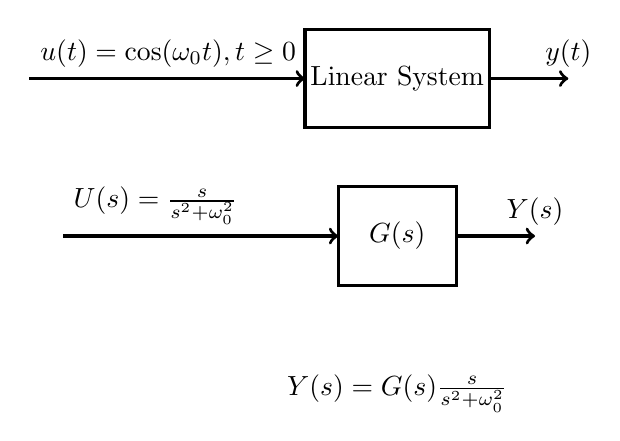
\begin{tikzpicture}[inner sep=0pt,outer sep=0pt,very thick,
sysblock/.style={draw,rectangle,inner sep=2pt,minimum width=1.5cm,minimum height=1.25cm,very thick}]
\draw (0,2) node[sysblock] (G1) {Linear System};
\draw[<-] (G1.180) -- ++(-3.5,0) node[above right=4pt] {$u(t) = \cos(\omega_{0}t), t \geq 0$};
\draw[->] (G1.0) -- ++(1,0) node[above=4pt] {$y(t)$};


\draw (0,0) node[sysblock] (G) {$G(s)$};
\draw[<-] (G.180) -- ++(-3.5,0) node[above right=4pt] {$U(s)=\frac{s}{s^{2}+\omega_{0}^{2}}$};
\draw[->] (G.0) -- ++(1,0) node[above=4pt] {$Y(s)$};

\draw (0,-2) node {$Y(s) = G(s)\frac{s}{s^{2}+\omega_{0}^{2}}$};
\end{tikzpicture}

\end{center}
\end{frame}

\begin{frame}{Step 2: Write partial fraction expansion, splitting poles at $\pm j\omega_{0}$}
\begin{itemize}
\item Let $p_{1},p_{2}, \cdots, p_{n}$ be the poles of $G(s)$ (assume simple poles for now, but result also holds if $G(s)$ has repeated poles)
\[
Y(s) = G(s)\frac{s}{s^{2}+\omega_{0}^{2}} = \frac{A}{s-j\omega_{0}} + \frac{B}{s+j\omega_{0}} + \frac{C}{s-p_{1}} + \frac{D}{s-p_{2}} + \cdots
\]
\item By residue formula
\begin{align*}
A &= \left.\cancel{(s-j\omega_{0})}G(s)\frac{s}{\cancel{(s-j\omega_{0})}(s+j\omega_{0})}\right|_{s=j\omega_{0}} = G(j\omega_{0})\frac{1}{2}\\
B &= \left.\cancel{(s+j\omega_{0})}G(s)\frac{s}{(s-j\omega_{0})\cancel{(s+j\omega_{0})}}\right|_{s=-j\omega_{0}} = G(-j\omega_{0})\frac{1}{2}\\
\end{align*}
\end{itemize}
\end{frame}

\begin{frame}{Step 3: Find Inverse Laplace Transform}
\begin{itemize}
\item Since
\[
Y(s) = \frac{ G(j\omega_{0})\frac{1}{2}}{s-j\omega_{0}} + \frac{G(-j\omega_{0})\frac{1}{2}}{s+j\omega_{0}} + \frac{C}{s-p_{1}} + \frac{D}{s-p_{2}} + \cdots
\]
\item Using $e^{-at}\step  \overset{\mathcal{L}}{\longleftrightarrow} \frac{1}{a+s}$ the time response is
\[
y(t) =\left(G(j\omega_{0})\frac{1}{2}e^{j\omega_{0}t} + G(-j\omega_{0})\frac{1}{2}e^{-j\omega_{0}t}+Ce^{p_{1}t} + De^{p_{2}t}\right)u(t)
\]
\end{itemize}
\end{frame}

\begin{frame}{Step 4: Use property of stable poles}
\begin{itemize}
\item If $\mbox{Re}(p_{i})=-a<0$, 
\[
\lim_{t\rightarrow \infty} Ce^{p_{i}t}u(t) = \lim_{t\rightarrow \infty} Ce^{\mbox{Re}(p_{i})t}e^{j\mbox{Im}(p_{i})t}u(t)=\lim_{t\rightarrow \infty} Ce^{-at}e^{j\mbox{Im}(p_{i})t}u(t) = 0
\]
\item Thus
\[
\lim_{t\rightarrow \infty} y(t) =\left(G(j\omega_{0})\frac{1}{2}e^{j\omega_{0}t} + G(-j\omega_{0})\frac{1}{2}e^{-j\omega_{0} t}\right)
\]
\end{itemize}
\end{frame}

\begin{frame}{Step 5: Use symmetry property $G(-j\omega)=G(j\omega)^{*}$ and Euler's formula}
\begin{itemize}
\item Substitute for $G(-j\omega_{0})$
\[
\lim_{t\rightarrow \infty} y(t) =\left(\frac{1}{2}G(j\omega_{0})e^{j\omega_{0}t} + \frac{1}{2}G(j\omega_{0})^{*}e^{-j\omega_{0} t}\right)
\]
\item Write in polar form, using $a^{*}=|a|e^{-j\angle a}$
\[
\lim_{t\rightarrow \infty} y(t) =\left(\frac{1}{2}|G(j\omega_{0})|e^{j\angle G(j\omega_{0})}e^{j\omega_{0}t} + \frac{1}{2}|G(j\omega_{0})|e^{-j\angle G(j\omega_{0})}e^{-j\omega_{0} t}\right)
\]
\item Euler's formula: $\frac{1}{2}Ae^{j\theta} + \frac{1}{2}Ae^{-j\theta} = A\cos(\theta)$
\[
\lim_{t\rightarrow \infty} y(t) = |G(j\omega_{0})|\cos(\omega_{0}t + \angle G(j\omega_{0}))
\]
\end{itemize}
\end{frame}
What we have shown is if the input is a cosine with frequency $\omega_{0}$, then the output, at steady state, is also a cosine with frequency $\omega_{0}$, but with an amplitude gain of $G(j\omega_{0})$, and a phase shift of $\angle G(j\omega_{0})$. This is summarized below in the general case.

\begin{frame}{Sinusoidal Steady State is the Frequency Response}
\begin{theorem}
Given a stable system with transfer function $G(s)$, the sinusoidal steady state response is defined by the input/output relationship
\[
\boxed{\begin{aligned}
u(t) & = A\cos(\omega_{0}t + \theta), \\
y_{ss}(t) & = |G(j\omega_{0})|A\cos\left(\omega_{0}t + \theta + \angle G(j\omega_{0})\right).
\end{aligned}
}
\]
\end{theorem}
\begin{definition}
$G(j\omega)$ is the {\em frequency response function} of the system with transfer function $G(s)$.
\end{definition}
\end{frame}

Note: since $\sin(\omega t) = \cos(\omega t - 90^{\circ})$ the same is true for sine functions.

\section{Examples}

\begin{example} Find the steady state response
\begin{align*}
G(s) &= \frac{1}{s+1}\\
u(t) & = 3\cos(2t + 30^{\circ}), t \geq 0
\end{align*}
\textbf{Solution:} Calculate the magnitude and phase of $G(j2)$:
\begin{center}
\begin{minipage}{2in}\begin{align*}
|G(j2)| &= \left|\frac{1}{j2+1}\right|\\
&= \frac{|1|}{|j2+1|} \\
& = \frac{1}{\sqrt{1+2^2}} \\
& = \frac{1}{\sqrt{5}}
\end{align*}
\end{minipage}
\begin{minipage}{2in}\begin{align*}
\angle G(j2) &= \angle \frac{1}{j2+1}\\
&= \angle 1 - \angle j2+1 \\
& = 0 - \tan^{-1}\left(\frac{2}{1}\right) \\
& = -63.4^{\circ}
\end{align*}
\end{minipage}
\end{center}
The solution is thus
\[
y_{ss}(t) = \frac{3}{\sqrt{5}}\cos(2t - 33.4^{\circ})
\]


\end{example} 
\begin{example}
Find an expression for the magnitude and phase frequency response functions for a system with transfer function
\[
G(s) = \frac{\sigma}{s+\sigma}
\]
where $\sigma>0$. 
\textbf{Solution:}
The magnitude of the frequency response function is given by
\begin{align*}
|G(j\omega)| &= \left|\frac{\sigma}{j\omega+\sigma}\right| \\
& = \frac{|\sigma|}{|j\omega + \sigma |} \\
& = \frac{\sigma}{\sqrt{\omega^{2}+\sigma^{2}}}
\end{align*}
The phase of the frequency response function is given by
\begin{align*}
\angle G(j\omega) &= \angle \frac{\sigma}{j\omega+\sigma} \\
& = \angle\sigma  -\angle (j\omega + \sigma) \\
& = 0 - \tan^{-1}\left(\frac{\omega}{\sigma}\right)\\
& = -\tan^{-1}\left(\frac{\omega}{\sigma}\right)
\end{align*}

\end{example}

\section{Lecture Highlights}
The primary takeaways from this article include
\begin{enumerate}
\setlength{\itemsep}{5pt}
\setlength{\parskip}{0pt}
\setlength{\parsep}{0pt}
\item After an initial transient response period, the output of a dynamic system with a sinusoidal input will be a steady-state sinusoid that has the same frequency $\omega_0$ as the input signal.
\item The output sinusoid will be scaled (amplitude changed) and shifted (phase angle changed) according to properties of the system's transfer function $G(s)$.
\item By evaluating the magnitude and phase angle of the system's transfer function $G(s)$ at $s = j \omega_0$, we can determine the steady-state output signal without having to go through the full inverse Laplace transform process.
\end{enumerate}

\section{Quiz Yourself}

\subsection{Questions}

\begin{enumerate}
\setlength{\itemsep}{5pt}
\setlength{\parskip}{0pt}
\setlength{\parsep}{0pt}
\item The following system models a transmission line
\begin{center}
\input{quizfigures/circuitproblem1.tex}
\end{center}
and has the transfer function
\[
\frac{V_{out}(s)}{V_{in}(s)} = \frac{1}{4s^{2}+8s+3}
\]
Find the steady state output if the following sinusoids are applied as input
\begin{enumerate}
\item $\cos(0.1 t)$
\item $\cos(t)$
\item $\cos(10t)$
\end{enumerate}
\end{enumerate}

\subsection{Solutions}
\begin{enumerate}
\setlength{\itemsep}{5pt}
\setlength{\parskip}{0pt}
\setlength{\parsep}{0pt}
\item[1(a)] \rule{12pt}{0pt}
\begin{center}
\includegraphics[width=5in]{quizfigures/1asoln}
\end{center}
\item[1(b)]\rule{12pt}{0pt}
\begin{center}
\includegraphics[width=5in]{quizfigures/1bsoln}
\end{center}
\newpage
\item[1(c)]\rule{12pt}{0pt}
\begin{center}
\includegraphics[width=5in]{quizfigures/1csoln}
\end{center}
\end{enumerate}



\end{document}


